\documentclass{deutez}
\DeclareUnicodeCharacter{202F}{\,}
\usepackage{placeins}%resim kaymaları için kullanıldı FloatBarrier
\newcommand\tab[1][1cm]{\hspace*{#1}}
\usepackage{xcolor}
\usepackage{graphicx}
\usepackage{amsmath,amsthm,mathtools}
\usepackage{iftex}
\pagestyle{empty}

\ifTUTeX
\usepackage{fontspec}
\else
\usepackage[T1]{fontenc}
\usepackage[utf8]{inputenc} % The default since 2018
\DeclareUnicodeCharacter{200B}{{\hskip 0pt}}
\fi
%\documentclass{standalone}
%%%%%%%%%%%%%%%%%%%%%GANTCHART%%%%%%%%%%%%%%%%%%%%%%%%%%%%%%%%%
\usepackage{adjustbox}
\usepackage{color}
\usepackage{tikz}
\usepackage{pgfgantt}
\usepackage{pdflscape}%gantchart içim
\newganttchartelement{orangebar}{
	orangebar/.style={
		inner sep=0pt,
		draw=red!66!black,
		very thick,
		top color=white,
		bottom color=orange!80
	},
	orangebar label font=\huge,
	orangebar left shift=.1,
	orangebar right shift=-.1
}

\newganttchartelement{bluebar}{
	bluebar/.style={
		inner sep=0pt,
		draw=purple!44!black,
		very thick,
		top color=white,
		bottom color=blue!80
	},
	bluebar label font=\huge,
	bluebar left shift=.1,
	bluebar right shift=-.1
}

\newganttchartelement{greenbar}{
	greenbar/.style={
		inner sep=0pt,
		draw=green!50!black,
		very thick,
		top color=white,
		bottom color=green!80
	},
	greenbar label font=\huge,
	greenbar left shift=.1,
	greenbar right shift=-.1
}

\newganttchartelement{redbar}{
	redbar/.style={
		inner sep=0pt,
		draw=red!90!black,
		very thick,
		top color=white,
		bottom color=red!90
	},
	redbar label font=\huge,
	redbar left shift=.1,
	redbar right shift=-.1
}

\newganttchartelement{blackbar}{
	blackbar/.style={
		inner sep=0pt,
		draw=black!90!black,
		very thick,
		top color=white,
		bottom color=black!90
	},
	blackbar label font=\huge,
	blackbar left shift=.1,
	blackbar right shift=-.1
}

%%%%%%%%%%%%%%%%%%%%%%%%%%%%%%%%%%%%%%%%%%%%%%%%%%%%%%%%%%%%%%%%%%%%%%%%%%%%%%%%%%%%%%%%%%
\graphicspath{ {./images/} }
\watermarklogo{Deu.jpg}  % Dokuz Eylül Üniversitesi Logosu; Sayfaya arkasına varsayılan logo olarak basılır.

\projectname{Smart Mirror Controller}%
\ogrencininadi{Rabia DOĞAN}%
\advisor{Ph.D. Özgür TAMER}%
\time{January,2021}%

\begin{document}
	\start
	
	\begin{abstract}	
	\paragraph~In the project, general purpose is to give the Smart Mirror controllable features with hand gestures. In this way, the product will be able to appeal to the upper customer segments and increase its market share. The main goal here is to enable users to use most of the smart mirror applications with hand movements, to eliminate the need to touch the mirror, thus to eliminate the contamination in the touched parts of the mirrors and therefore to possible dissatisfaction with the product and to ensure that the product can be used even in cases where the users cannot touch the mirror with their hands for various reasons, such as the bathroom. Although camera-based systems are generally used for gesture recognition, it will not be welcomed by many users to have a camera in a personal use area such as the bathroom.Therefore, passive infrared sensor arrays will be preferred for gesture recognition in our project. They can be preferred in application areas where cameras are relatively weak because they work with the infrared radiation emitted by living creatures. We aim to detect hand gesture and then the movement of the hand gesture. In this way, gesture distinction can be made with a simpler electronic design with less processing load and lower cost than a standard camera. The project is carried out and supported by Vestel Elektronik A.Ş. with the code TEYDEB 3170688. 
	\end{abstract}
	
	\begin{ozet}
	\paragraph~	Projede genel amaç Akıllı Aynaya el jestleri ile kontrol edilebilir özellikler kazandırmaktır.Bu sayede ürün üst müşteri segmentlerine de hitap edebilecek, pazar payını artırabilecektir.Burada temel hedef kullanıcıların akıllı ayna uygulamalarının birçoğunu el hareketleri ile kullanabilmesini sağlayarak, aynaya dokunma ihtiyacını ortadan kaldırmak böylece aynaların dokunulan bölgelerindeki kirlenmeyi ve dolayısıyla da ürün ile ilgili olası memnuniyetsizliği	ortadan kaldırmak ve banyo gibi kullanıcıların çeşitli nedenler ile elleri ile aynaya dokunamayacakları durumlarda dahi ürünün kullanılabilmesini sağlamaktır.Jest tanıma için genellikle kamera temelli sistemler kullanılmakla beraber, banyo gibi kişisel kullanıma dönük bir alanda kamera 	bulunması birçok kullanıcı tarafından hoş karşılanmayacaktır.Bu nedenle projemizde jest tanımlama amacıyla pasif kızılötesi sensör dizileri tercih edilecektir.Bu tip sensörler oldukça düşük çözünürlüklerde görev yapmasına karşın, nesne ya da canlıların yaydığı kızılötesi ışıma ile çalıştıkları için kameraların görece zayıf kaldığı uygulama alanlarında tercih edilebilmektedirler.Pasif kızılötesi sensörler ile öncelikle kullanıcının jestini ve	sonrasında da jestin hareketini algılamayı amaçlamaktayız.Bu sayede standart bir kameraya göre daha az işlem yükü ve daha düşük maliyet ve	daha basit bir elektronik tasarım ile jest ayrımı yapılabilecektir.	Proje Vestel Elektronik A.Ş.taarafından TEYDEB 3170688 kodu ile yürütülmekte ve desteklenmektedir.
	\end{ozet}
	\tableofcontents
	\listoffigures
	\listoftables
	\chapter{Introduction}	
	\paragraph~	The general purpose of the project is to add a gesture detection system to the Smart Mirror at the cheapest cost. 
	\paragraph~	One of the most important issues in the project where privacy is prioritized is the selection of sensors. One of the best choices for this is the use of a thermopile array sensor. It is a system that measures infrared radiation, developed with the thermocouple method dating back to 150 years. A thermocouple consists of 4 ends, there are two different materials connected to 2 ends, while the other two ends are connected to a voltage meter\cite{htpa}. If an absorber is attached to the junction and exposed to the effect of IR radiation from an object, the thermocouple junction heats up due to the incoming radiation while the absorber collects incoming heat\cite{htpa}. The thermocouple material in turn converts the temperature difference voltage indicated by the voltmeter. Hence, the voltmeter reading is a direct measure for object temperature. This method is simple, does not require any mechanics and can detect static signals accurately\cite{htpa}.
	\paragraph~Before Smart Mirror integration, it was decided to use an external microcontroller. The reason for this was that the processor in the Smart Mirror did not work very well. It was decided to go to an external card selection so that the process would not be extended and the project delivery could be achieved within the specified time. The sensor PCB to be developed should be designed to connect the sensor to the microcontroller and to receive data from the sensor in the most efficient way. The sensor and microcontroller to be selected will show us the path to follow.
	\paragraph~	For the development of the software chapter, the software language most suitable for the project will be preferred. Detection of appropriate gestures for the Thermopile array sensor, microcontroller and intelligent Mirror are elements that will affect the selection of the software language for the project. The first step is to retrieve data from the sensor. After the successful acquisition of this, in the resulting image, the human body and all objects in the background emit infrared radiation. Therefore, the sensor also detects these objects. This problem can be solved by threshold methods in the literature. The simple threshold method returns the same threshold value for each pixel. Pixel values less than the threshold value are changed to 0\cite{opencv}. The adaptive threshold is the method by which the threshold value is calculated for smaller regions, and therefore there will be different threshold values for different regions\cite{opencv}. Another method is Otsu's method. It is also a type of adaptive threshing. Instead of selecting a threshold value, Otsu's method automatically determines it \cite{image}.
	\paragraph~4 Static and 4 dynamic movements are the gestures we currently set for a smart mirror. There are some methods that will help us understand whether movements are dynamic or static. With the Barycenter method, it is possible to adopt a similar case of planetary motions for gestures \cite{car}. Another method is MHI (memory History Image)\cite{mhi}. A comparison is made by taking images with certain time intervals. The difference between images shows us that movement exists.
	\paragraph~The next step, classification methods should be performed to match the acquired image with the previously specified commands. Some methods are as follows; \\
	Hybrid Method (the combination of Haar-Like and HOG features ) is a feature extraction method. Using this method after, multi-class SVM(Support Vector Machine ) is used for final hand gesture recognition \cite{hybrid}.  HOG(Histogram of Oriented Gradient) features is one of the feature extraction methods. After applying this method, hand recognition is to find the matched image in the database. Using nearest-neighbour algorithms, this step is carried out. \cite{HOG}. k-NN(k-nearest neighbour); It is one of the most popular machine learning algorithms because it is resistant to old, simple and noisy training data. However, it also has a disadvantage. Overlap, it is necessary to get up-to-date information required for big data that we store in the long term. There are database sets. Then, by using the fall detection algorithm, the object in front is distinguished with the other objects. Finally, k-NN classification is made using the data in the database\cite{KNN}. CNN (convolutional neural networks) is one of the most commonly used algorithms for image classification. An image classifier takes a photo or video as input and classifies it into one of the possible categories it is trained to identify.\cite{CNN1}\cite{CNN2} \cite{car}.
	\paragraph~All that remains is communication between the selected microcontroller and Smart Mirror.
	
	\chapter{Methodology}
	\paragraph~In this section, the methods to be applied in the project are included.
	\begin{figure}[h!]
		\centering
		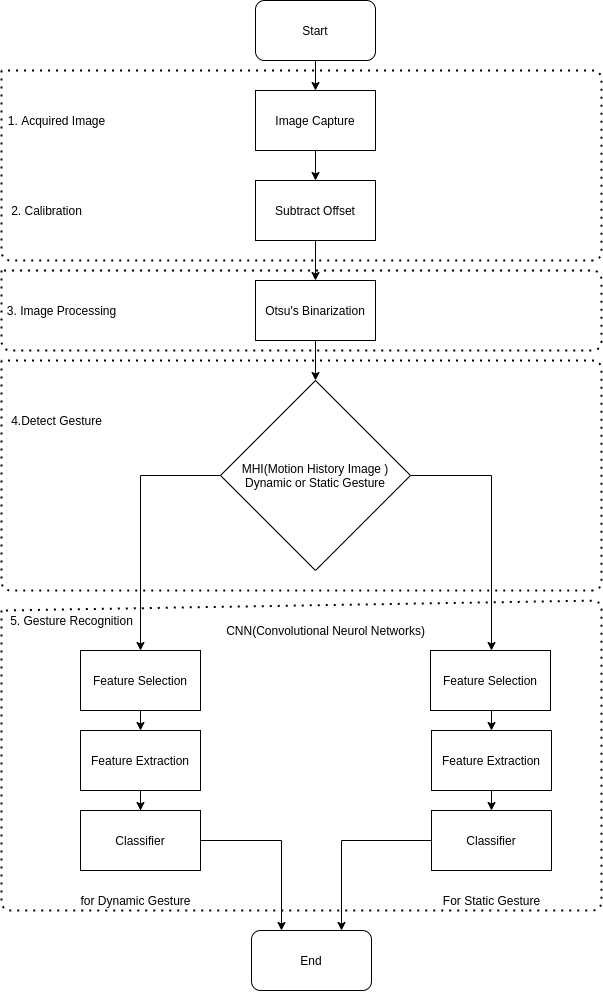
\includegraphics[width=0.75\textwidth]{şema}
		\caption{Software Flowchart}
	\end{figure}
	\FloatBarrier
	\section{Capture Thermopiles Image}
\paragraph~	The sensor chosen to be used in the project is HTPA32x32d thermopile array sensor. HTPA32x32d thermopile array sensor 32x32 pixel, operates between -10 and 70 degrees, provides I2C communication, has an internal EEPROM and provides an 8-bit data set. EEPROM data contains calibration data for each pixel of the sensor.
	\begin{figure}[h!]
		\centering
		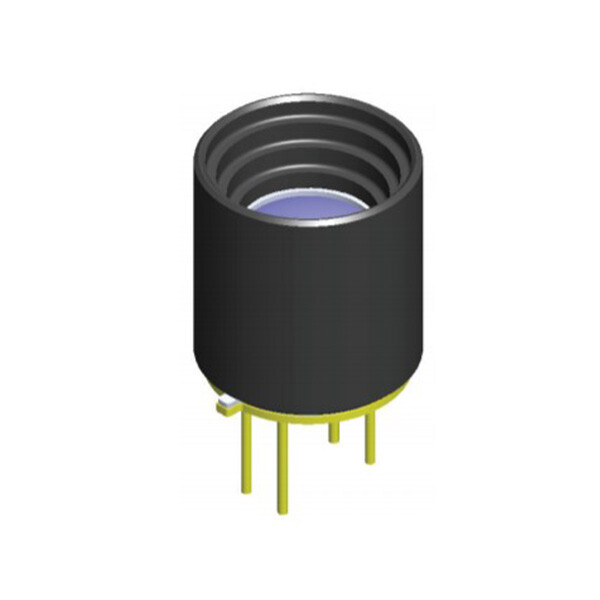
\includegraphics[width=0.35\textwidth]{htpa}
		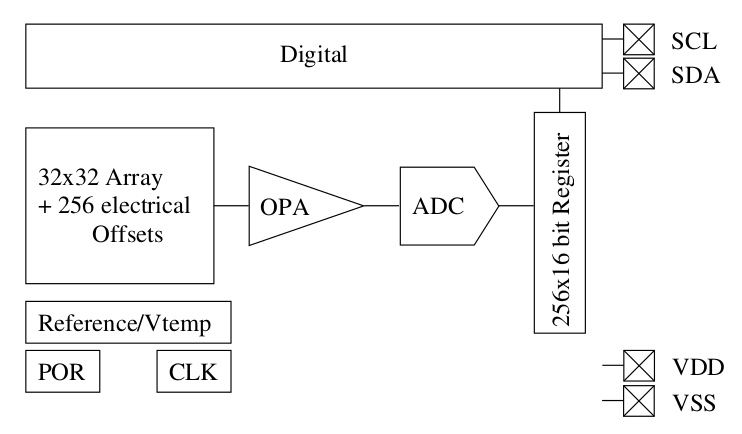
\includegraphics[width=0.60\textwidth]{htpasema}
		\caption{Schematic for HTPA32x32d}
	\end{figure}
	\FloatBarrier
\paragraph~	The sensor uses 7-bit I2C address 0x1A for configuration and sensor data and 7-bit I2C address 0x50 to access internal EEPROM. The address byte is followed by a W / R bit and an 8-bit command.\\
	To read data from the chip first the address and read command must be sent. After the last ACK, a new start-bit (repeated start) and the address with a set read-flag initiates the read sequence. There can be bytes read as many as required. The last byte must be denoted by a not-acknowledge.\\
	\begin{figure}[h!]
		\centering
		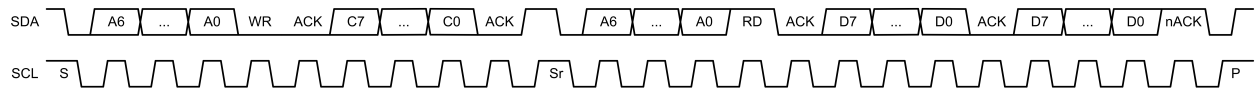
\includegraphics[width=1\textwidth]{read_data}
		\caption{Read Command}
	\end{figure}
	\FloatBarrier
\paragraph~	The sensor is divided into two parts (Top and Bottom Half), which are also divided into 4 blocks. The reading order is shown below for different blocks. When a conversion is initiated, the X Block of the upper and lower half are measured simultaneously. Each block consists of 128 Pixels sampled entirely in parallel. The reading order in the lower half is mirrored compared to the upper half so the center lines are always read last.
	\begin{table}[h!]
		\begin{center}
			\caption{Read Data 1 Command (Top Half of Array)}
			\begin{tabular}{|c|c|c|c|c|c|c|c|c|} 
				\hline
				Addr/CMD & \multicolumn{8}{c|}{0x1A (7 Bit!) / 0x0A}\\\cline{1-9}
				Read Data &7&6&5&4&3&2&1&0\\
				\cline{1-9}
				1. Byte / 2. Byte & \multicolumn{8}{c|}{PTAT 1 MSB / LSB or Vdd 1 MSB / LSB}\\\cline{1-9}
				3. Byte / 4. Byte & \multicolumn{8}{c|}{Pixel (0+BLOCK*128) MSB / LSB}\\\cline{1-9}
				5. Byte / 6. Byte & \multicolumn{8}{c|}{Pixel (1+BLOCK*128) MSB / LSB}\\\cline{1-9}
				... & \multicolumn{8}{c|}{}\\\cline{1-9}	
				257. Byte / 258. Byte & \multicolumn{8}{c|}{Pixel (127+BLOCK*128) MSB / LSB}\\\cline{1-9}
				
			\end{tabular}
		\end{center}
	\end{table}
	\FloatBarrier
	\begin{table}[h!]
		\begin{center}
			\caption{Read Data 2 Command (Bottom Half of Array)}
			\begin{tabular}{|c|c|c|c|c|c|c|c|c|} 
				\hline
				Addr/CMD & \multicolumn{8}{c|}{0x1A (7 Bit!) / 0x0B}\\\cline{1-9}
				Read Data &7&6&5&4&3&2&1&0\\
				\cline{1-9}
				1. Byte / 2. Byte & \multicolumn{8}{c|}{PTAT 2 MSB / LSB or Vdd 2 MSB / LSB}\\\cline{1-9}
				3. Byte / 4. Byte & \multicolumn{8}{c|}{Pixel (992-BLOCK*128) MSB / LSB}\\\cline{1-9}
				5. Byte / 6. Byte & \multicolumn{8}{c|}{Pixel (993-BLOCK*128) MSB / LSB}\\\cline{1-9}
				... & \multicolumn{8}{c|}{}\\\cline{1-9}	
				65. Byte / 66. Byte & \multicolumn{8}{c|}{Pixel (1023-BLOCK*128) MSB / LSB}\\\cline{1-9}
				
				65. Byte / 66. Byte & \multicolumn{8}{c|}{Pixel (1023-BLOCK*128) MSB / LSB}\\\cline{1-9}
				
				67. Byte / 68. Byte & \multicolumn{8}{c|}{Pixel (960-BLOCK*128) MSB / LSB}\\\cline{1-9}
				
				69. Byte / 70. Byte & \multicolumn{8}{c|}{Pixel (961-BLOCK*128) MSB / LSB}\\\cline{1-9}
				
				... & \multicolumn{8}{c|}{}\\\cline{1-9}
				
				129. Byte / 130. Byte & \multicolumn{8}{c|}{Pixel (991-BLOCK*128) MSB / LSB}\\\cline{1-9}
				
				131. Byte / 132. Byte & \multicolumn{8}{c|}{Pixel (928-BLOCK*128) MSB / LSB}\\\cline{1-9}
				
				...& \multicolumn{8}{c|}{}\\\cline{1-9}
				
				257. Byte / 258. Bytes& \multicolumn{8}{c|}{Pixel (927-BLOCK*128) MSB / LSB}\\\cline{1-9}
				
			\end{tabular}
		\end{center}
	\end{table}
	\FloatBarrier
\paragraph~	Complete sensor data must be read at once. If communication falls somewhere in between, all successive data will be corrupted. Reading can be stopped anywhere by pausing the clock. A newly started reading progress through this stopped byte, continuing the clock, but the index is reset when a new conversion is started. If the bit for electrical offsets (Bit 1 in Config 0x01) is set, the electrical offsets are sampled and can be read similar to the active pixel.
\paragraph~	After reading the data in blocks, there are a few more steps we need to take.Object and ambient temperature can be calculated from sensor output and stored calibration data. The figure below shows an overview of the EEPROM in Figure 2.2.
	\begin{figure}[h!]
		\centering
		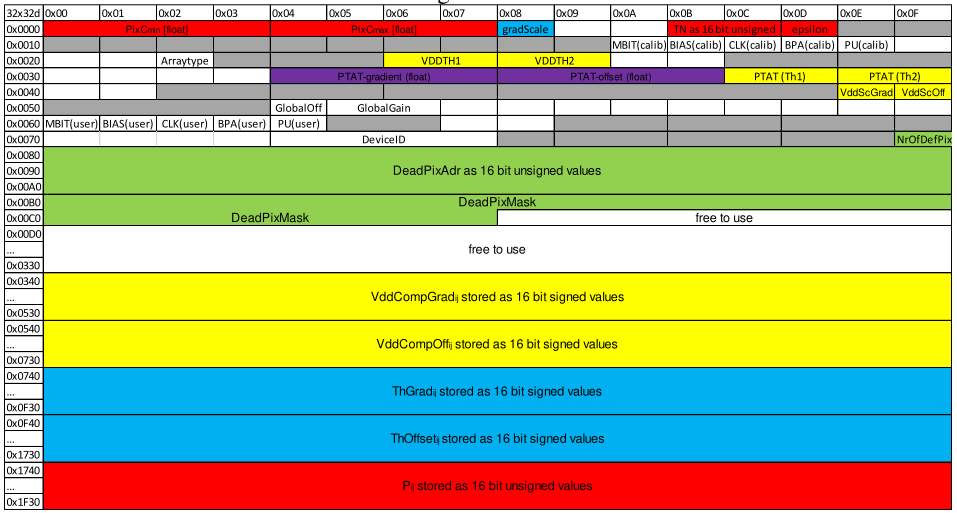
\includegraphics[width=0.8\textwidth]{eeprom}
		\caption{EEPROM overview 32x32d}
	\end{figure}
	\FloatBarrier
\paragraph~	Unless otherwise specified, all values are stored as unsigned 8-bit values. Small endian format is used for larger values. Fields marked in gray are used during calibration or for future use and the Heimann Sensor is reserved. \\
	The ambient temperature (Ta) is calculated from equation 2.1
	\begin{equation}
	T_a=PTAT_{av} \cdot PTAT_{gradient}+ PTAT_{offset}
	\end{equation}
	where:\\
	$ \mathbf{PTAT_{av}} = \frac{\sum \limits _{i=0}^{7}{PTAT_i}}{8} $ is the average measured PTAT value.\\
	$\mathbf{PTAT_{gradient}}$ and $\mathbf{PTAT_{offset}}$ are from EEPROM.
\paragraph~	The thermal offset of sensor has to be subtracted for each pixel to compensate for any thermal deviation.
	\begin{equation}
	V{ij_Comp}=V{ij}-\frac{Th_{Gradij} \cdot T_a}{2^{gradScale}}-Th_{Offset_{ij}}
	\end{equation}
	where:\\
	\textbf{ij}	represents the row (i) and column (j) of the pixel.\\
	$\mathbf{V_{ijComp}} $		is the thermal offset compensated voltage.\\
	$\mathbf{V_{ij}}  $ is the raw pixel data (digital), readout from the RAM.\\
	$\mathbf{Th_{Gradij}}$		is the thermal gradient, stored in the EEPROM from 0x740 to 0xF3F.\\
	$\mathbf{Th_{Offsetij}}$		is the thermal offset, stored in the EEPROM from 0xF40 to 0x173F.\\
	$\textbf{gradScale}$		 is the scaling coefficient for the thermal gradient stored in the EEPROM.
	\paragraph~	Electrical stabilization is used to compensate for changes in supply voltage. This compensation is only one subtraction, so it can be done before or after thermal offset compensation. We chose to do it later.\\
	The compensation for the top half is done by using the following formula:\\
	\begin{equation}
	V_{ijComp}^{\ast} =V_{ijComp}-elOffset[(j+i\cdot 32)]\%128]
	\end{equation}
	The bottom half analogue with this formula:\\
	\begin{equation}
	V_{ijComp}^{\ast} =V_{ijComp}-elOffset[(j+i\cdot 32)]\%128+128]
	\end{equation}
	where:\\
	\textbf{ij} represents the row (i) and column (j) of the pixel and electrical offset.\\
	$\mathbf{V_{ijComp}^{\ast}}$ is the thermal and electrical offset compensated voltage.\\
	$\mathbf{V_{ijComp}}$ is the $\textbf{elOffset[ij]}$ thermal offset compensated voltage.\\
	$\mathbf{elOffset[ij]} $
	is the electrical offset belonging to Pixel ij.\\
	A supply voltage compensation called $ Vdd_{Comp}  $is used to provide supply voltage changes. To use this compensation, the sensor's supply voltage (Vdd) must be measured by the sensor, adjusting the configuration record and averaging from time to time. $Vdd_1$ and $Vdd_2$ result in Vdd.Average Voltage is calculated by equation 2.5.\\
	\begin{equation}
	VDD_{av}=\frac{\sum \limits _{i=0} ^{7}{VDD_i}}{8}
	\end{equation}
	Compensation for the Top half is done using the formula:\\
	\begin{multline}
	V_{ij-VDD_{Comp}}=V_{ij-VDD{Comp}}^{\ast}-\\
	\frac{\frac{Vdd_{CompGrad}[(j+i\cdot 32)\%128]\cdot PTAT_av}{2^{Vdd_{ScGrad}}}+V_{Vdd_{Compoff}}[(j+i\cdot 32)\%128]}{2^{Vdd_{ScOff}}}\\
	\cdot(VDD_av-VDD_{TH1}-(\frac{VDD_{TH2}-VDD_{TH1}}{PTAT_{TH2}-PTAT_{TH1}})\cdot(PTAT_{av}-PTAT_{TH1}))
	\end{multline}
	The bottom half analogue with this formula:\\
	\begin{multline}
	V_{ij-VDDComp}=V_{ij-VDDComp}^{\ast}-\\
	\frac{\frac{Vdd_{CompGrad}[(j+i\cdot 32)\%128+128]\cdot PTATav}{2^{Vdd_{ScGrad}}}+V_{Vdd_{Compoff}}[(j+i\cdot 32)\%128+128]}{2^{Vdd_{ScOff}}}\\\cdot(VDD_av-VDD_{TH1}-(\frac{VDD_{TH2}-VDD_{TH1}}{PTAT_{TH2}-PTAT_{TH1}})\cdot(PTAT_av-PTAT_{TH1}))
	\end{multline}
	where:\\
	$ \textbf{ij} $ represents the row (i) and column (j) of the pixel.\\
	$ \mathbf{V_{ij-VDDComp}}$ is the Vdd compensated voltage.\\
	$ \mathbf{V_{ij-VDDComp}}^{\ast} $ is the thermal and electrical offset compensated voltage.\\
	$ \mathbf{Vdd_{CompGrad}[ij]} $ is the VddComp gradient belonging to Pixel ij.\\
	$ \mathbf{Vdd_{CompOff}[ij]} $ is the VddComp  belonging to Pixel ij.\\
	$ \mathbf{VDD_{av}} $ is the average measured supply voltage of the sensor in Digits.\\
	$ \mathbf{Vdd_{ScGrad}} $ is a scaling coefficient and stored in the EEPROM 0x4E.\\
	$ \mathbf{Vdd_{Scoff}} $ is a scaling coefficient and stored in the EEPROM 0x4F.\\
	$ \mathbf{VDD_{TH1}} $ is the supply voltage during calibration 1 stored in the EEPROM 0x26, 0x27.\\
	$ \mathbf{VDD_{TH2}} $ is the supply voltage during calibration 2 stored in the EEPROM 0x28, 0x29.\\
	$ \mathbf{PTAT_{TH1}} $ is the PTAT value of calibration 1 stored in the EEPROM 0x3C, 0x3D.\\
	$ \mathbf{PTAT_{TH2}} $ is the PTAT value of calibration 2 stored in the EEPROM 0x3E, 0x3F.
	
\paragraph~	All we need to do to get the thermal image and separate it is to do the above given mathematical operations and steps. For this we will use a python library periphery-python.
	After reading the data from our sensor, after applying the steps of thermal offset, electrical offset and Vdd Compensation, the data will appear in all its simplicity.
\paragraph~	\textbf{NOTE:All steps to acquired the image are made with reference to the datasheet\cite{datasheet}.}
	
	\section{Hand Thermal Image Isolation}
\paragraph~	Our biggest advantage in the project is that our sensor is infrared, so only the objects that emit heat are detected. The main purpose in this section is to separate the hand from the back body. The hand is in front of the body will cause us to perceive the hand warmer. For this reason, the body with hand will appear as two different objects. The second step is to pull the hand off the background. There are many methods for this today. Among these methods, we decided to use OTSU's Method.
	According to this method, "it approaches the feasibility of directly evaluating the "goodness" of the threshold and automatically selecting the most suitable threshold"\cite{Otsu1}.\\You can see an example of an image with Otsu's method applied in the figure 4.1.
	\paragraph~Formuluzation:
	the gray level histogram is normalized and regarded as a probability distribution:\\
	\begin{equation}
	p_i=\frac{n_i}{N} , p_i \geq 0, {\sum \limits _{i=1} ^{L}{p_i}}
	\end{equation}
	Where:\\
	$ N=n_1 +n_2 +...n_{1024} $ total number of pixel\\
	
	\paragraph~Let's divide the pixels into two class as CO and C1 with a threshold, where CO represents the background while C1 represents the foreground. Suppose we call our Threshold Value k.The set C0 implies the background pixels with a gray level of [1, ...,k], and C1 means those pixels of foreground object with a gray level of [k + 1, . . . , L]. The probabilities of gray level distributions for the two class are the following: $  \omega_0  $is the probability of the background and $ \omega_1 $ is the probability of the object\cite{Otsu2}.\\
	\begin{figure}[h!]
		\centering
		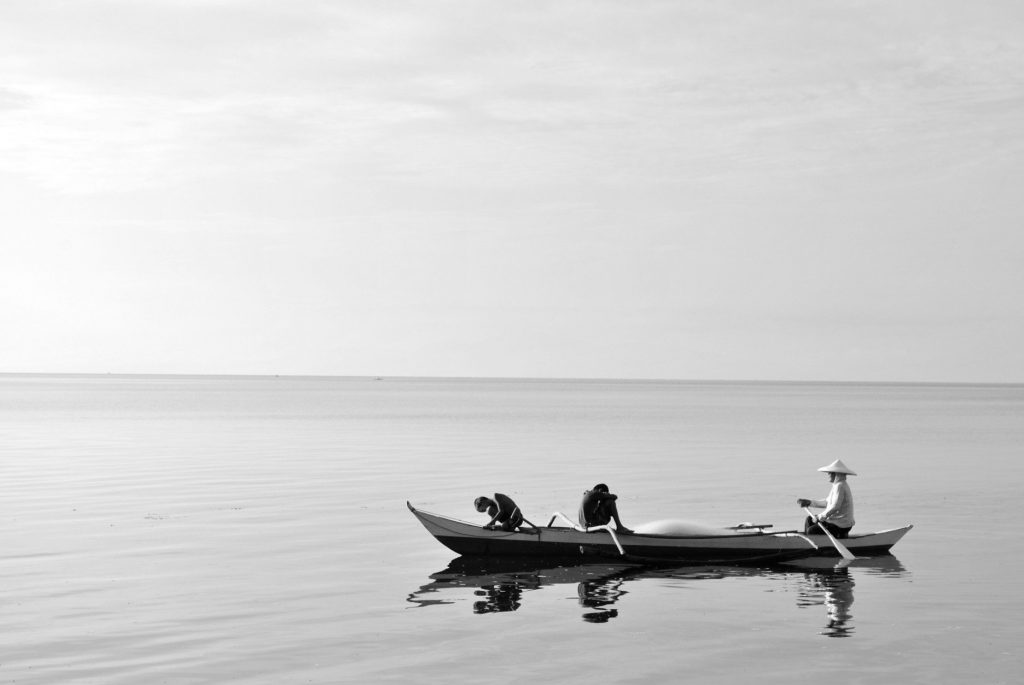
\includegraphics[width=0.32\textwidth]{otsu1}
		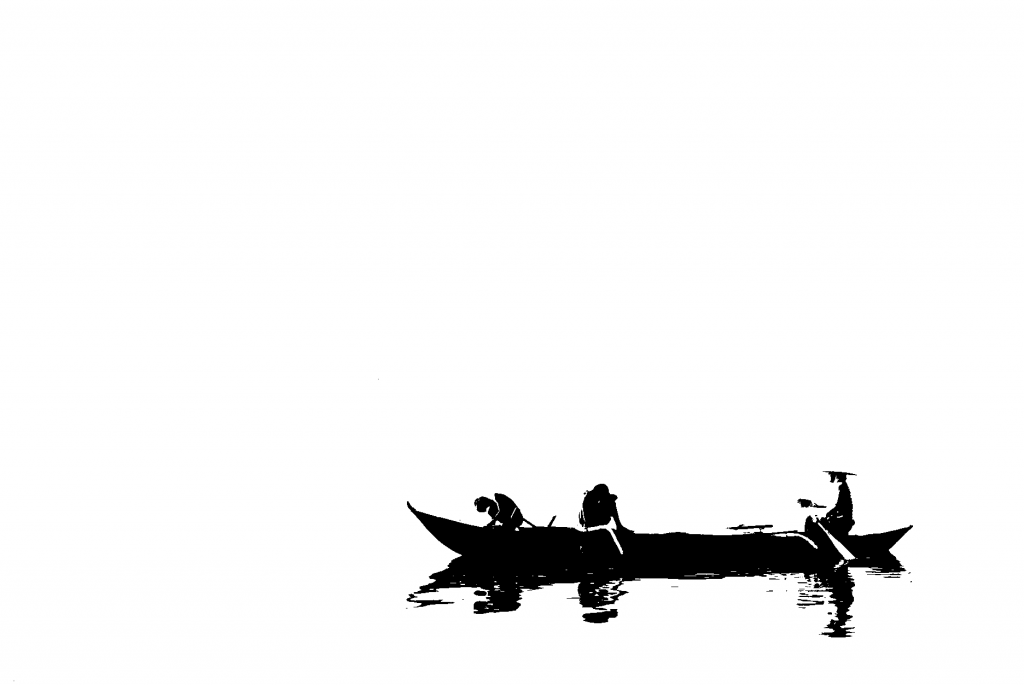
\includegraphics[width=0.3\textwidth]{otsu2}
		\caption{Application of Otsu's method}
	\end{figure}
	\FloatBarrier
	
	\begin{equation}
	\omega_0=P_r(C_0)={\sum \limits _{i=1} ^{k}{p_i}}=\omega (k)
	\end{equation}
	
	\begin{equation}
	\omega_1=P_r(C_1)={\sum \limits _{i=k+1} ^{L}{p_i}}=1-\omega(k)
	\end{equation}
	and 
	\begin{equation}
	\mu_0={\sum \limits _{i=1} ^{k}{i P_r (i|C_0)}}={\sum \limits _{i=1} ^{k}{\dfrac{i p_i}{\omega_0}}}=\frac{\mu(k)}{\omega(k)}
	\end{equation}
	
	\begin{equation}
	\mu_1={\sum \limits _{i=k+1} ^{L}{i P_r (i|C_1)}}={\sum \limits _{i=k+1} ^{L}{\dfrac{i p_i}{\omega_1}}}=\frac{\mu_r- \mu(k)}{1-\omega (k)}
	\end{equation}
	where:\\
	\begin{equation}
	\omega_k={\sum \limits _{i=1} ^{k}{p_i}}
	\end{equation}
	
	\begin{equation}
	\mu_k={\sum \limits _{i=1} ^{k}{i p_i}}
	\end{equation}
\paragraph~	Cumulative of the zeroth- and first-order cumulative moments of the histogram:\\
	\begin{equation}
	\mu_T=\mu(L)={\sum \limits _{i=1} ^{L}{i p_i}}
	\end{equation}
	\paragraph~It is the total average level of the original picture. For any choice of k, we can easily verify the following relationship:\cite{Otsu1}
	\begin{equation}
	\omega_0 \mu_0 +\omega_1 + \mu_1 =\mu_T, \tab \omega_0 + \omega_1=1
	\end{equation}
	\paragraph~Calculated the class variance:
	\begin{equation}
	\sigma_0^2={\sum \limits _{i=1} ^{k}{(i-\mu_0)^2P_r(i|C_0)}}={\sum\limits_{i=1}^{k}{(i-\mu_0)^2}\frac{p_i}{\omega_0}}
	\end{equation}
	\begin{equation}
	\sigma_1^2={\sum \limits _{i=k+1} ^{L}{(i-\mu_1)^2P_r(i|C_1)}}={\sum\limits_{i=k+1}^{L}{(i-\mu_1)^2}\frac{p_i}{\omega_1}}
	\end{equation}
	\paragraph~Between-class variance is:
	
	\begin{equation}
	\sigma_B^2=\omega_0(\mu_0-\mu_T)^2+\omega_1(\mu_1-\mu_T)^2=\omega_0\omega_1(\mu_0-\mu_1)^2
	\end{equation}
	\paragraph~Within class Variance is:
	\begin{equation}
	\sigma_W^2=\omega_0\mu_0^2+\omega_1\mu_1^2
	\end{equation}
	\paragraph~Total Varience:
	\begin{equation}
	\sigma_T^2=\sigma_W^2+\sigma_B^2
	\end{equation}
	\paragraph~Calculated Otsu threshold:
	\begin{equation}
	\sigma_B^2{(k)}=\frac{[\mu_T\omega(k)-\mu(k)]^2}{\omega(k)[1-\omega(k)]}
	\end{equation}
	\paragraph~and optimal threshold $ k^* $ is:
	\begin{equation}
	\sigma_B^2(k^*)=\max\limits_{1\leq k<L}{\sigma_B^2(k)}
	\end{equation}
	\paragraph~After these procedures, we have a threshold value. When we ignore the parts below this threshold and take the parts above, we will see a clear hand shape.
	\paragraph~If we cannot perceive the hand clearly as a result of the Otsu method, then the
	Using the Neighbor contour detection algorithm, we can make the image what we want\cite{Otsu2}.
	\FloatBarrier
	\section{Hand Gesture Recognition}
	\paragraph~Motion history image (MHI) helps in understanding the template location and path as motion progresses in a static image. In MHI, temporal motion information is narrowed down to a single image pattern where intensity is a function of the novelty of motion. Hence, the MHI pixel density is a function of motion history at that location where brighter values correspond to a newer motion\cite{MHIbook}.Using MHI method in the project, the information will be obtained whether the gestures are static or dynamic.
	Take two continuous frames. Some noise, background image, moving object information for the captured images in functions.
	\begin{equation}
	\begin{gathered}
	I(x,y,t)=b_t (x, y) + m_t (x, y) + n_t (x, y)\\
	I (x, y, t + 1) = b_{t+1} (x, y) + m_{t+1} (x, y) + n_{t+1} (x, y)
	\end{gathered}
	\end{equation}
	where,\\
	$ \mathbf{b_t (x, y) }$: Static background for t th frame.\\
	$ \mathbf{m _t (x, y) }$: Moving objects for t th frame.\\
	$ \mathbf{n _t (x, y)} $: Background noise for t th frame.\\
	
	%%%%%%%%%%%%%%5
	\begin{equation}
	\begin{gathered}
	diff(x, y, t) = I(x, y, t + 1)-I(x, y,t)\\
	diff (x, y, t) = b(x, y) + md(x, y, t) + nd(x, y, t)
	\end{gathered}
	\end{equation}
	where,\\
$ \mathbf{	b(x, y, t)} $: Overlapped area in consecutive frames.\\
$ \mathbf{	md(x, y, t)} $: Motion region.\\
$ \mathbf{	nd(x, y, t) }$: Noise (which can be ignored based on situations).\\
	If there is no movement, it will be defined as no movement, since this difference will be 0\cite{MHIbook}.
	\subsection{Static Gesture Recognition}
\paragraph~	Deep learning techniques have emerged recently and advances in convolutional neural networks (CNN) surpass the classical approach to hand gesture recognition as it eliminates the need to derive complex handcrafted features from images\cite{gesturecnn}.CNN's automate the feature extraction process by learning high-level abstractions in images and capturing the most distinguishing feature values using the hierarchical architecture. Thus, it solves the disadvantage of obtaining inconsistent property descriptors when working with large numbers of motion classes with very small cross-class variations\cite{static}.
\paragraph~	Convolution layer,"Each image of a picture is processed by convolution, and the width and length of the image are compressed to obtain deeper image information"\cite{gesturecnn}.
\paragraph~	Pooling layer,"study found that every time when the convolution, convolution may be missing information, pool layer can solve this problem. No compression when the convolution aspect at the same time, to retain more information,compressed work on completion of the pool floor"\cite{gesturecnn}.
	
	\begin{figure}[h!]
		\centering
		\includegraphics[width=1\textwidth]{CNN1}
		\caption{The architecture of a typical CNN\cite{static}.}
	\end{figure}
	\FloatBarrier
\paragraph~	"Deep learning is an extension of the neural network architecture that automates the process of extracting features from meta data by operating through a series of hierarchical layers"\cite{static}. The project aims to use such a deep learning architecture that uses a convolutional neural network to recognize static hand gestures. Convolution layers contain units called feature maps, each of which is linked to local patches in the previous layer via filter sets\cite{LeCun}. The same filterbank is used in all units of a feature map, and different filter banks are used in different feature maps in one layer. This architecture allows us to easily identify local patterns distinctive from images, even if they are in different parts of the image\cite{LeCun}.
	\begin{figure}[h!]
		\centering
		\includegraphics[width=0.7\textwidth]{CNN2}
		\caption{The Schematic Representation of the Proposed CNN model for hand posture recognition\cite{static}.}
	\end{figure}
	\FloatBarrier
\paragraph~	The locally weighted sum obtained by the filtering process is filtered and filtered through a nonlinear function called ReLu (Flattened Linear Unit) to stabilize the convolved results. The pooling process is included in the CNN structure to group semantically similar properties from the convolution layer. Thus, the architecture of a CNN includes two or three convolution layers, then more convolutional layers with linear activation and pooling layers, followed by pooling and activation, and a fully connected final layer that performs classification\cite{static}.
	\subsection{Dynamic Gesture Recognition}
\paragraph~Unlike static motion, dynamic motion requires both hand shape and hand motion.The main idea at this stage is to take the coordinates of the manually tracked centre in each frame. These coordinates will be used to know which mirror command corresponds to which movement \cite{dynamic}. The coordinates will be used differently for each movement depending on the perceived hand gestures. 4 of the 8 hand gestures are used for dynamic hand movements. These dynamic hand gestures are categorized as unidirectional and versatile hand gestures. Currently, only one-way movements are defined in this project. One-way hand gestures require the shape of the hand and the direction of movement to command.


	\section{Matching Gesture to Commands of Smart Mirror}
\paragraph~	A number of scenarios have been prepared for command mapping for smart mirror. The scenarios prepared are as follows;
\paragraph~	For Static Gestures:\\
	We have 4 fixed gestures. It is the ability to Open, Close, Touch and Return to the Home Page.\\
	\begin{figure}[h!]
		\centering
		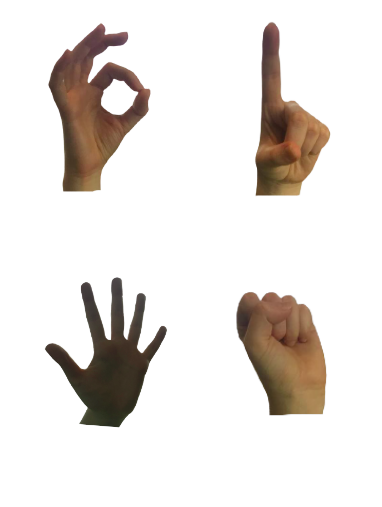
\includegraphics[width=0.27\textwidth]{tek2}
		\caption{Gestures of Open,Close,Touch,Return to the Home Page }
	\end{figure}
	\FloatBarrier
	For Dynamic Gestures:\\
	There are two mobile situations. Down-Up, Right-Left properties.
	\begin{figure}[h!]
		\centering
		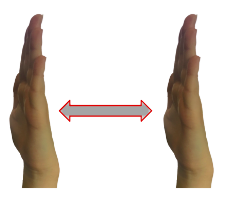
\includegraphics[width=0.27\textwidth]{tek}		
		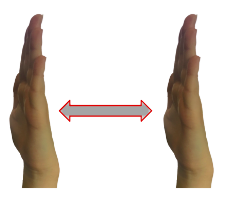
\includegraphics[width=0.27\textwidth,angle=90]{tek}
		\caption{Gestures of Down-up, Right-Left }
	\end{figure}
	\FloatBarrier
\paragraph~	In total, we activated 8 features of the smart mirror with gesture.Afterthat, by activating the Raspberry Pi OTG communication channel, intelligent Mirror and MCU communication is provided.
	\section{Sensor and MCU Communication PCB Design}
\paragraph~	A sensor PCB design will be made with the selection and supply of the passive infrared sensor. In the PCB design in question, a schematic design will be made first and the necessary components and connections will be made schematically. After this part, the schematic design will be turned into a printed circuit. In the design of the printed circuit board, along with the schematic design, the physical properties of the place where the sensor will be mounted will be taken into consideration in the current smart mirror design. After this part, the designed sensor PCB will be produced in an external company and its assembly will be carried out in the company.\\
	The pcb and schematic drawings of the communication PCB are as shown in the figures below. Schematic and PCB design will be done using KiCad EDA - Schematic Capture \& PCB Design Software. In the next step, support will be received for printed circuit operations. After soldering the printed cards, our sensor communication PCB will be ready and the test phase will begin. \\
	\begin{figure}[h!]
		\centering
		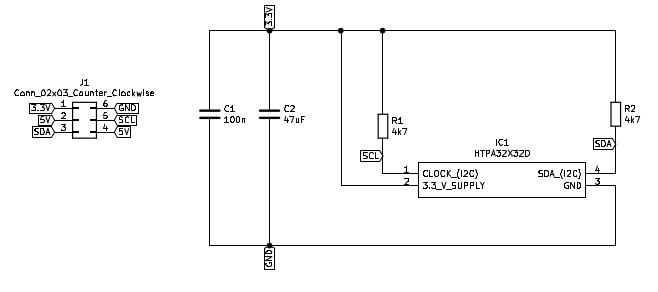
\includegraphics[width=0.7\textwidth]{schematic}
		\caption{Schematic Design of Communication PCB}
	\end{figure}
	\FloatBarrier
	\begin{figure}[h!]
		\centering
		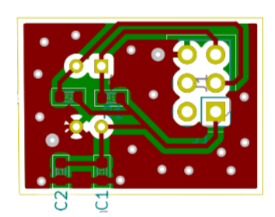
\includegraphics[width=0.4\textwidth]{pcb}
		\caption{PCB Design of Communication PCB}
	\end{figure}
	\FloatBarrier
	
	\chapter{Work Plan and Work Packages}
	\begin{table}[h!]
		\begin{adjustbox}{width=\textwidth}
			\begin{tabular}{|l|}\hline
				Worker:Rabia DOĞAN   \tab[8cm] Time: 7 Weeks (2020.10.01-2021.01.15)\\\hline
				Work Package Name:Literature Review and Material Supply\\\hline
				Inputs:\\
				• Past studies.\\
				• Articles on internet.\\
				• Thesis on internet.\\
				• Books.\\\hline	
				Steps:•\\ Searching for articles Gesture Recognition with Infrared array sensor. \\
				•Searching the OpenCV library and Python programming language.\\
				•Searching convenential neural network for gesture recognition \\
				•Searching Thermopil Array sensors\\\hline
				Outputs:\\
				•Determining Thermopil Array Sensor.\\ 
				•Determining methods to be used.\\\hline
				Status:Complated.\\\hline
			\end{tabular}
		\end{adjustbox}
	\end{table}
	\FloatBarrier
	\begin{table}[h!]
		\begin{adjustbox}{width=\textwidth}
			\begin{tabular}{|l|}\hline
				Worker:Rabia DOĞAN   \tab[8cm] Time: 3 Weeks (2021.01.11-2021.02.03)\\\hline
				Work Package Name:Sensor PCB Design\\\hline
				Inputs:\\
				•HTPA32x32d Application Notes \\\hline	
				Steps :\\
				•Drawing Schematic Design\\
				•Drawing PCB Design\\
				•Testing Sensor PCB\\\hline
				Outputs:\\
				•Schematic and PCB Design of Sensor PCB.\\\hline
				Status:In Progress\\\hline
			\end{tabular}
		\end{adjustbox}
	\end{table}
	\FloatBarrier
	\begin{table}[h!]
		\begin{adjustbox}{width=\textwidth}
			\begin{tabular}{|l|}\hline
				Worker:Rabia DOĞAN   \tab[8cm] Time: 9 Weeks (2021.01.03-2021.03.15)\\\hline
				Work Package Name:Gesture Detection\\\hline
				Inputs:\\
				•Methods of Gesture Recognition\\
				•HTPA32x32d Datasheet\\
				•Books about of Image Processing\\\hline	
				Steps :\\
				•Reading sensor data with the help of the python-periphery library.\\
				•Making calibrations with EEPROM calibration data.\\
				•Removing the hand from the background with the Herbaceous Method.\\
				•Hand condition detection with Motion History Image method.\\
				•Defining gesture with CNN\\
				Outputs:\\
				• Capture sensor Image\\
				•Detected Gesture Types \\
				•Tracking Gesture Recognition \\
				•Matching Gesture to Commands of Smart Mirror\\\hline
				Status:In Progress\\\hline
			\end{tabular}
		\end{adjustbox}
	\end{table}
	\newpage
	\begin{table}[h!]
		\begin{adjustbox}{width=\textwidth}
			\begin{tabular}{|l|}\hline
				Worker:Rabia DOĞAN   \tab[8cm] Time: 3 Weeks (2021.03.16-22.03.30)\\\hline
				Work Package Name:Smart Mirror and Sensor PCB Integration\\\hline
				Inputs:\\
				•WP1,WP2,WP3 outputs \\\hline	
				Steps : \\
				•Connectting Raspberry pi and Smart Mirror with OTG Communication\\\hline
				Outputs:\\
				•Complated the project\\\hline
				Status:In Progress\\\hline
			\end{tabular}
		\end{adjustbox}
	\end{table}
	\FloatBarrier
	\begin{landscape}
		\noindent\resizebox{260mm}{!}{\begin{ganttchart}[
				hgrid style/.style={black, dotted},
				vgrid={*5{black,dotted}, *1{white, dotted}, *1{black, dashed}},
				x unit=2mm,
				y unit chart=9mm,
				y unit title=12mm,
				time slot format=isodate,
				group label font=\bfseries \Huge,
				link/.style={->, thick}
				]{2020-10-01}{2021-03-30}
				\gantttitlecalendar{year, month=name, week}\\
				
				\ganttgroup[
				group/.append style={fill=orange}
				]{Literature Review and Material Supply}{2020-10-01}{2021-01-15}\\ [grid]
				\ganttorangebar[
				name=Documentation
				]{Literature Review}{2020-10-01}{2021-01-15}\\ [grid]
				\ganttorangebar[
				name=FMETutorial
				]{Material Supply}{2020-12-01}{2021-01-15}\\ [grid]
				%%%%%%%%%%WP2%%%%%%%%%%%%
				\ganttgroup[
				group/.append style={fill=blue}
				]{Sensor PCB Design}{2021-01-11}{2021-02-03}\\ [grid]
				
				\ganttbluebar[
				name=FMETutorial
				]{Referance Circuit Rewiev}{2021-01-11}{2021-01-13}\\ [grid]
				\ganttlinkedblackbar{}{2021-01-13}{2021-01-14}
				\ganttbluebar[
				name=FMETutorial
				]{Schematic Design}{2021-01-14}{2021-01-15}\\ [grid]
				
				\ganttlinkedblackbar{}{2021-01-15}{2021-01-16}
				\ganttbluebar[
				name=FMETutorial
				]{PCB Design}{2021-01-16}{2021-01-18}\\ [grid]
				
				\ganttlinkedbluebar{}{2021-01-18}{2021-02-01}
				
				\ganttbluebar[
				name=FMETutorial
				]{Testing Sensor PCB}{2021-02-01}{2021-02-03}\\ [grid]
				%%%%%%%%%%%%%%%%%%%WP3%%%%%%%%%%%%%%%%%%%%%%%%%%%%%%
				\ganttgroup[
				group/.append style={fill=red}
				]{Gesture Detection}{2021-01-03}{2021-02-15}\\ [grid]
				%\ganttredbar[
				%name=FMETutorial
				%]{Hand Thermal Image Isolation}{2020-01-03}{2021-01-21}\\ [grid]
				\ganttredbar[
				name=FMETutorial
				]{Receiving Data From The Sensor}{2021-01-03}{2021-01-05}\\ [grid]
				\ganttlinkedblackbar{}{2021-01-05}{2021-01-06}
				\ganttredbar[
				name=FMETutorial
				]{Making The Data Meaningful}{2021-01-06}{2021-01-07}\\ [grid]
				\ganttlinkedblackbar{}{2021-01-07}{2021-01-08}
				\ganttredbar[
				name=FMETutorial
				]{Isolation of The Hand From The Data Received From the Sensor}{2021-01-08}{2021-01-18}\\ [grid]
				\ganttlinkedblackbar{}{2021-01-18}{2021-01-19}
				\ganttredbar[
				name=FMETutorial
				]{Detecting Hand Condition}{2021-01-19}{2021-01-30}\\ [grid]
				\ganttlinkedblackbar{}{2021-01-30}{2021-02-15}
				\ganttredbar[
				name=FMETutorial
				]{Tracking Hand Movement}{2021-02-15}{2021-03-15}\\ [grid]
				
				%%%%%%%%%%%%%%%%%%WP4%%%%%%%%%%
				\ganttgroup[
				group/.append style={fill=green}
				]{Smart Mirror and Sensor PCB Integration}{2021-03-16}{2021-03-30}\\ [grid]
				\ganttgreenbar[
				name=FMETutorial
				]{Communication Hardware Implementation}{2021-03-16}{2021-03-21}\\ [grid]
				\ganttlinkedblackbar{}{2021-03-21}{2021-03-26}
				\ganttgreenbar[
				name=FMETutorial
				]{Communication Software Implementation}{2021-03-16}{2021-03-21}\\ [grid]
				\ganttlinkedblackbar{}{2021-03-21}{2021-03-22}
				
				\ganttgreenbar[
				name=FMETutorial
				]{Sensor PCB, Smart Mirror Integration}{2021-03-22}{2021-03-28}\\ [grid]
				
				\ganttgreenbar[
				name=FMETutorial
				]{Detect Gesture as Gesture Command}{2021-03-28}{2021-03-30}\\ [grid]
		\end{ganttchart}}
	\end{landscape}
	\chapter{Cost Analysis}
	\section{Economical Costs}
\paragraph~	In this project, the economic cost is only in the hardware part. A Raspberry Pi 4B and Thermopil array sensor are used in our project. The market price of Raspberry Pi 4B is \$55. The thermopil array sensor, on the other hand, has been chosen the most suitable for our project and has been researched for the market. The price of the HEIMANN HTPA32x32d Thermopil array sensor is \$87. There is currently no separate cost in the software part. Because using opensource software.
	\section{Environmental,Political and Social Costs}
\paragraph~	Infrared sensor arrays have emerged in recent years and are products that allow the application of thermal imaging technologies to consumer electronics. With the introduction of Covid-19 into our lives, it is frequently encountered in the field of thermal imaging. Since a consumer electronics product using these products has not been produced in Turkey yet, it is considered to contribute to the national knowledge. In the project where privacy is prioritized, the privacy of the person will be ensured by using a thermopile array sensor. Also, the project is executed by Vestel A.Ş. so the project is expected to inspire different projects within Vestel. The fact that these sensors are newly introduced to the market will pave the way for innovative applications in many fields and thus method changes that can turn into patents. For example, although gesture recognition is performed with cameras conventionally, it offers a significant innovation in methodology, using passive infrared arrays. Smart mirrors that can be controlled with gesture recognition can have a positive effect on the preference of the products in question by the consumers. In doing so, using a technology that does not impair personal privacy will ensure that the users put the product into their lives safely and the applications related to the product become widespread.
	\chapter{Conclusion}
\paragraph~	The reason for the project is that the system made with the existing infrared sensors does not work as desired. The main purpose of the system is to renew the smart mirror again to appeal to the upper segments. 8 features have been defined for the new gesture detection system that we will add to the smart mirror. However, if the device is desired to be released to the market, the number of transactions can be increased without touching the smart mirror by increasing the gesture suggestions.
\paragraph~	The Thermocouple system, which dates back to a very old past, is becoming increasingly popular today. Based on this formation, it was decided to use the Thermopile array sensor, aiming both to prevent reflections around and aim at the confidentiality of privacy. The most important points in determining the sensor are the frame rate and the pixel value to make the image clearer. The conclusion reached in the research based on these two properties was the use of the HEIMANN HTPA32x32d sensor. Also the project needs a processor. While the tablet processor in the Smart Mirror was assumed to be sufficient at the first stage, it was later concluded that the performance of the tablet processor was insufficient for this project. While moving on to the Raspberry Pi, the Raspberry family, which is one step ahead in price-performance comparison in the market, is considered sufficient for the project in terms of speed and operating system.
\paragraph~	Image acquisition was the next step. At this stage, the periphery-python library in the python language to get the image comes to the fore with its ability to read large pixels and give fast results. If we assume that the image taken is an offset image, the offset values ​​are calculated and stored separately for each pixel via EEPROM, which is one of the advantages of the selected sensor. With the data received from the EEPROM address, the image is finally in the clearest form. Thermopil array sensors detect all objects that emit infrared rays, so it is necessary to isolate the hand from the background image. The Otsu method, which is the most advanced of adaptive thresholding methods, is one of the techniques that will yield the best results for this project. Now there is only a hand shape in the image. In the system with 8 gestures, it is possible to separate two as Static and Dynamic gestures. The not too complicated MHI (Motion History Image) method will be used to distinguish between the two types of gestures. By comparing the images taken as two frame sets, it will be understood whether there is a difference or not, and whether the image will be dynamic or static will be distinguished. Two separate CNN (convenantial neurol network) clasification algorithms will be implemented for dynamic and static images. Among the image classification methods, it is the CNN method that stands out for gesture detection. Finally, the Raspbery Pi and Smart mirror will be integrated. Looking at the project, the most innovative methods will be used on the basis of the method to be used.
	\bibliographystyle{deueeebst2.bst}
	\bibliography{refs}
	
\end{document}